 \documentclass[16pt,a4paper]{article}
 \usepackage{amsmath}
 \usepackage{graphicx}
 \usepackage{xcolor}
 \usepackage{fixltx2e}
 \usepackage{hyperref}
 \usepackage{wrapfig}
\usepackage{multirow}
\begin{document}
 \begin{wrapfigure} {r} {0.1\textwidth}
 	\vspace{-60pt}
    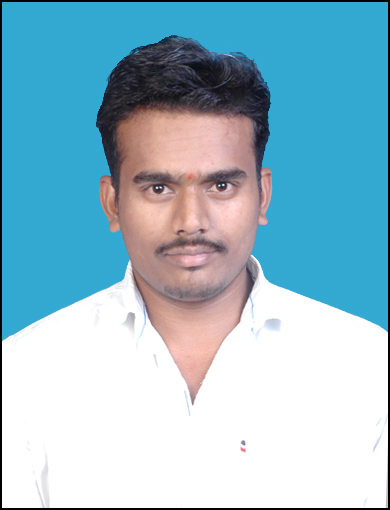
\includegraphics[width=3cm,height=4cm]{said.jpg}
 \end{wrapfigure}
        \textbf{Name:}Sachin Mahadev Jadhav\\
        \textbf{Address:} At Itti, Post-Poharegaon, Tal: Renapur,\\ Dist: Latur, Pin - 413512.\\
        \textbf{Contact NO:}9850823263\\
        \textbf{E-mail:} {jadhavsa996@gmail.com} 
       \begin{center}
       	 \line(1,0){450}
       \end{center}
     \section{Career Objective:} 
 	  Utilization of knowledge and Technical skills along with design abilities to promote growth and development of the organization and self by implementing my innovative ideas, skills and creativity.
   \begin{center}
   	\line(1,0){450}
   \end{center}
 \section{Academic Details:} 
\begin{tabular}{||c|l|c|r|l|l||}
	\hline
	Sr No:& Class & Year of Passing  & institute &Grades \\
	\hline
	1.&	TY B.Tech & 2017-18 &\multirow{3}{*}{WCE,Sangli}&9.3  \\
	2.&	SY B.Tech & 2016-17 &  &9.12 \\
	3.&	FY B.Tech & 2015-16 &  &8.78 \\
	4.&	HSC & 2014-15 & Dayanand Science college,Latur &91.38 \\
	5.&	SSC & 2012-13 & Renuka Vidyalay Bhokaramba &91.45 \\
	\hline
\end{tabular}
\begin{center}
	\line(1,0){450}
\end{center}

%%%%%%%%%%%%%%%%%%%%%%%%%%%%%%%%%%%%%%%%%%%%%%%%			
\section{Projects Undertaken:} 
\begin{enumerate}
	
	\item Biomorphic Hyper Redundant Snake Robot.
	\begin{description}
		\item [$\bullet$]Under E-Yantra 2017 robotic competition organized by IITB.\\
		-Using joystick communication and 3D designing of snake and Servo actuator.
	\end{description}
	\item  Line following based multipurpose system for hospitals.
	\begin{itemize}
		\item India innovation challenge design contest by Texas Instruments and IIM Bangalore.
		\item	Idea is to make clone for doing multiple tasks such as sweeping,cleaning,dustbin collection,medicine delivery
	\end{itemize}
	\item Pocket DSO
	\begin{description}
		\item [$\bullet$]Third  year sem 2 miniproject
		\item [$\bullet$]Cost and Power efficient portable DSO using GLCD with MSP430.\\
	\end{description}
	
	\item  Anti-pilferage and anti-adulteration system for fuel road tankers. 
	\begin{description}
		\item [$\bullet$] Smart India Hackthon 2018
		\item [$\bullet$]Solution to the pilferage and adulteration of fuel tanks en-route from terminals to retailer by continuous monitoring of location ,level, pressure and temperature parameters with cloud connectivity also ensuring emergency management. 
	\end{description}
	\item  Digital Trekking Watch.
	\begin{itemize}
		\item TY BTech sem 1 Mini project
		\item	OLED based compass and location tracking using magnetometer and GPS.
	\end{itemize}
	\item  Modeling 3D terrain in blender
	\begin{itemize}
		\item EYantra 2016 robotic championship by IITB
		\item 3D modelling of a terrain in Blender  using  X-bee comm. with \\Firebird V.
	\end{itemize}
\end{enumerate}
%%%%%%%%%%%%%%%%%%%%%%%%%%%%%%%%%%%%%%%%%%%%%%%%%%%%%%%%%%%%%%%%%
\section{Training and Workshop:} 
\begin{enumerate}
	\item Successfully completed the online course on Hardware Modelling Using Verilog conducted by \textbf{IIT KHARAGPUR} under NPTEL.
	\item Successfully compeleted workshop on \textbf{"Analog VLSI Design with Emphasis on OP-Amp Design"}.
\end{enumerate} 
\section{Technical skills:} 
\begin{enumerate}
	\item \textbf{Programing Skills:}
	\begin{itemize}
		\item C, Basic C++ and  Python.
		\item VHDL(Basic), VERILOG, Embedded C.
	\end{itemize}
	\item \textbf{Microcontrollers Known:}
	\begin{itemize}
		\item LPC2148 (ARM7),(low power microcontroller) MSP430G2553, MSP432P401R , P89V51RD2(8051), ATMEGA328P, ATmega2560.
	\end{itemize}
	\item \textbf{3D Designing Software:}
	Blender 2.7, Autodesk Fusion 360.
	\item \textbf{Simulation Software:}Proteus, Multisim 13,PSIM,VREP.
	\item \textbf{Firmware Orientation:}ATMEL 7.0, µvision 4 (keil), Code Compose \\Studio, Xillinx ISE 14.2.
	\item \textbf{PCB Designing Software:} Eagle 
\end{enumerate}
\section{EXTRA-CURRICULAR ACTIVITIES:}
\begin{enumerate}
	\item Coordinator of Cybermind committee in National level Technical Symposium \textbf{VISION 2K18} organized by WCE, Sangli.
	\item Currently working as Technical Director of \textbf{ELESA}.(ELectronics Engineering Student Association ).
	\item Also worked as Joint(2016-17) and Assistant(2015-16) Techincal director of \textbf{ELESA}.
\end{enumerate}
%%%%%%%%%%%%%%%%%%%%%%%%%%%%%%%%%%%%%%%%%%%%%%%
\section{CO-CURRICULAR ACTIVITIES:}
\begin{enumerate}
	\item 	Secured 4th rank with consolation prize in\textbf{E-yantra 2017 }National robotics competition organized by\textbf{ IIT Bombay}.
	\item	Currently shortlisted for second stage of \textbf {Smart India Hackathon 2018.}
	\item	Shortlisted in IICDC 2017 Quarterfinals organized by\textbf{ Texas instruments and IIM banglore} .
	\item	Semifinalist in E-Yantra 2016.	
\end{enumerate}
%%%%%%%%%%%%%%%%%%%%%%%%%%%%%%%%%%%%%%%%%%%%%%%%%%%
\section{ SOFT SKILLS:}
\begin{enumerate}
	\item 	Ability to work under pressure.
	\item lexibility, fast learning.
	\item	Good teamwork and Time management.	
\end{enumerate}

   \end {document}
   